% !TEX root = thesis.tex

\section{Classification of Log Data}\label{sec:layout}
TO BE FILLED

% \subsection{The title material}\label{sec:_title_material}
% The title of the report is printed in 16-pt bold.
% The title is fully capitalized, but use 14-pt capitals (or use `small caps') where lower-case letters would normally be used.
% Content words in the title must begin with a capital letter (`title caps').
% Leave 3 points of empty space under the title.

% The title is followed by the name of the author(s), with the student number(s) after the name.
% Note: remove the student number from the final version that you upload to the repository.
% Leave 6 points before the title, and 12 points after the last line.
% This is followed by the abstract.

% All the title details are centred on the page.

% \subsection{TO Be FILLED}\label{sec:_abstract_layout}
% The abstract should ideally consist of one paragraph containing a brief description of what is discussed in the document.
% Its maximum length is 250 words.
% Any further paragraphs in the abstract should have a 6 mm first-line indent, as in the main text.
% The abstract begins with the word Abstract (in bold), followed by a colon.
% After this comes the main text, beginning with a capital letter.

% The font size for the abstract is 9 pt.
% The abstract is presented as a single column across the whole page, with a 6 mm indent on both sides.
% The abstract is followed by 6 points of empty space, then the beginning of the main text.

% \subsection{The subheadings}\label{sec:_the_subeadings}
% It is advisable not to have more than two subheading levels in a short text.
% All subheadings should be in bold, numbered, with 12 points of empty space before them and 3 points after them.
% The font size for first-level subheadings is 12 pt.
% All other levels are 10 pt.
% Subheadings must be left-aligned.

% Arabic numerals should be used for subheadings.
% Single numbers (1, 2, etc.) are used for the first level, double numbers (1.1, 1.2 etc.) for the second level, three numbers for the third level, and so on.
% Numbers are followed by a full stop.

% Subheadings begin with a capital letter, but contain no further capitals.
% They do not end with a full stop.

% \subsection{The main text}\label{sec:_the_main_text}
% The main text was discussed in the first part of this section (10 pt, left and right aligned).
% It is advisable to check spelling and hyphenation.
% If you write Dutch in \LaTeX, you should \verb|\usepackage[dutch]{babel}|.
% Make sure there are no line breaks in the middle of formulae or between a number and unit (e.g.\ 6 cm).
% We strongly recommend that you use a spelling checker.
% Also check that tremas and accents, when required, are used correctly.

% Italics are used for words from other languages (except for terms that have become commonplace), Latin abbreviations, new terminology/concepts and for emphasis.
% Short quotes may also be italicized.
% Quotes must be placed between quotation marks.
% Make sure that you use opening and closing quotation marks correctly, i.e.\ `correct' and 'not correct' and ``also correct'' and ''wrong again''.

% The short dash - (hyphen) is used to join words or to separate the syllables of a word.
% The `en dash' is used as a minus sign and to indicate series of numbers ($-1$, $2 - 5$).
% The `em-dash' --- is used as a pause or parenthesis.

% Numbers are best presented using modified American notation, i.e.\ points are used where a comma would be used in Dutch, and vice versa.
% One and a half is therefore written as 1.5 and not as 1,5.
% Scientific notation should be used for large numbers: \SI{6.022e-23}.
% If necessary, spaces are used to separate large numbers into groups of three digits: $4 \; 294 \; 967 \; 296$.
% This also works after the decimal point: $3.141 \; 592 \; 653 \; 589 \; 79$.

% \subsection{Formulae}\label{sec:_formulae}
% Formulae must be written in the current notations used in mathematics, logic and physics.
% Make sure that symbols are properly explained.
% Use the same font as in the main text.
% % For LaTeX, avoid empty lines here which would lead to too much spacing above the equation!
% \begin{equation}\label{eq:some_formulae}
%   \delta J =  A \frac{dL}{dq} \delta q B + C \frac{dL}{dq} - \frac{d}{dt}\frac{dL}{dq} D~\delta q ~dt
% \end{equation}
% % An empty line and thus more space here is fine, but not if you continue your sentence after the formula.
% This equation can be referred to as equation~\ref{eq:some_formulae}, whereby the first number indicates the section and the second number is the number of the equation within the section.

% Formulae should be centred, and their numbers right-aligned.

% \subsection{Pseudocode}\label{sec:_pseudocode}
% It is best to express algorithms in pseudo code.
% This is a detailed high-level description using notations from mathematics and logic, and concepts from structured or object-oriented programming.

% The font size for pseudo code is 9 pt and, as with figures and tables, should be set apart from the main text.
% As in mathematical formulae, the names of  variables are italicized.
% Control words in the code (such as \textbf{if}, \textbf{then}, \textbf{else}, \textbf{for},\textbf{while}) should be in boldface.
% Function names (such as \textsc{Sort}, \textsc{FindShortest}, \textsc{ProcessSensor}, etc.) are printed in \emph{small caps}.
% Line numbers must be used if reference is made to individual lines of code.
% Blocks of code are indented, and conclude with end and the relevant control word, such as end for, end while or end else.

% When pseudo code is used, an explanatory caption must be included above the code.
% The caption should be 9 pt bold and begin with `Algorithm' followed by the section number and the number of the algorithm within the section.
% The reference to it in the text is `see algorithm~\ref{alg:some_algorithm}'.

% % see https://en.wikibooks.org/wiki/LaTeX/Algorithms_and_Pseudocode
% \begin{algorithm}[h]
% \caption{Calculate $y = x^n$}\label{alg:some_algorithm}
% \begin{algorithmic}
% \REQUIRE $n \geq 0 \vee x \neq 0$
% \ENSURE $y = x^n$
% \STATE $y \Leftarrow 1$
% \IF{$n < 0$}
% \STATE $X \Leftarrow 1 / x$
% \STATE $N \Leftarrow -n$
% \ELSE
% \STATE $X \Leftarrow x$
% \STATE $N \Leftarrow n$
% \ENDIF
% \WHILE{$N \neq 0$}
% \IF{$N$ is even}
% \STATE $X \Leftarrow X \times X$
% \STATE $N \Leftarrow N / 2$
% \ELSE[$N$ is odd]
% \STATE $y \Leftarrow y \times X$
% \STATE $N \Leftarrow N - 1$
% \ENDIF
% \ENDWHILE
% \end{algorithmic}
% \end{algorithm}

% \subsection{Figures}\label{sec:_figures}
% Figures must be comprehensible and the text they contain must be clearly legible.
% Bitmaps may only be used in the case of photos.
% They are not acceptable for line diagrams and graphs, unless the quality and resolution are so high that there is no visible difference.

% Graphs must have clear axes with the values marked, an indication of what they show and, where relevant, the units used.
% If more than one thing is shown in the graph, a legend must be provided or an explanation given in the caption below the graph.
% The various elements of the graph must be clearly distinguishable, even in black and white! Where relevant, graphs must also include reliability intervals or other information about possible variation.

% Figures must be either one or two columns wide, and must be placed either above or below the margins.

% An explanatory caption must be included below the figure.
% The caption begins with the word ‘Figure’, followed by the number of the section, a point and the number of the figure within the section.
% This is followed by a colon and the rest of the caption, beginning with a capital letter.
% The caption should be in 9-pt bold.
% Six points of blank space should be left between the caption of a figure and the text.

% The in-text reference is ‘see Figure 4.1’.
% Figures should be placed as close as possible to the first reference to them.

% \begin{figure}[h]
%   \centering
%   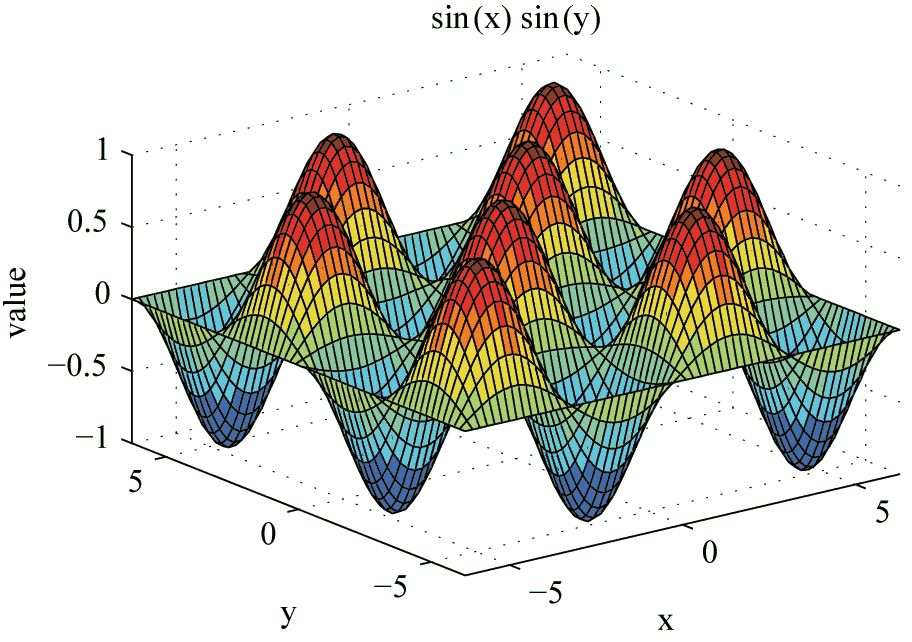
\includegraphics[width=\linewidth]{img/grafiek.png}
%   \caption{Graph of the function $sin(x) \cdot sin(y)$.
%     This figure is a bitmap, but of sufficiently high quality to be acceptable.
%     Take note of the legible axes and labels.
%   }\label{fig:afb1}
% \end{figure}

% \subsection{Tables}\label{sec_tables}
% Tables can be used if precise values are important, or in cases where a graph would not make things clearer.
% Tables may also be placed in the middle of the text if they are small enough.
% Otherwise, as with figures, they should be placed directly above or below the margin.

% A table consists of rows and columns.
% These must be clearly labelled (in bold).
% Numbers in a table are in ordinary typeface.
% The font size for all text in a table is 9 pt.
% Numbers are centred or aligned around the decimal point.
% In principle, rows and columns are separated by a single half-point line, but a certain amount of creativity may be used to group together related parts of the table.

% Tables must be provided with a caption (also 9-pt bold).
% Convention dictates that the caption should be \emph{placed} above the table.
% It begins with `Table', followed by the section number, a point, and the number of the table within the section.
% The in-text reference is `see Table~\ref{tab:some_table}'.
% One blank line is left above and below the table.
% It is also allowed to use Verdana 8 pt in the table if that is clearer.

% \begin{table}[h]
%   \centering
%   \caption{Number of student passes and fails per year.}\label{tab:some_table}
%   \begin{tabular}{llll}
%     \toprule
%     & 2003 & 2004 & 2005 \\
%     \midrule
%     passes & 16 & 19 & 17 \\
%     fails & 20 & 23 & 19 \\
%     \bottomrule
%   \end{tabular}
% \end{table}

% \subsection{References}\label{sec:_references}
% It is very important that the references in a document conform to a particular standard, because it must be possible for readers to find the background material referred to.
% The author, year, title of the book/journal, publisher and issue number must all be provided.
% This report should follow the conventions of the American Psychological Association.
% These can be found at \url{https://apastyle.apa.org/}, but it is usually more helpful to look at a number of examples.
% Other conventions may be used but this has to be discussed and approved of by your supervisor beforehand.
% To make it easier for your readers to access your references, please provide DOIs whenever possible --- you can search for them at \url{https://search.crossref.org/}.
% It is important to avoid references to vague sources as far as possible.
% It is best to avoid sources that are \emph{in press} or \emph{unpublished manuscripts}.
% For online resources which are not articles, always provide a \emph{complete and permanent URL} and mention the time you accessed them.

% In the text articles are referred to with the name(s) of the author(s) and the year \citep{dawkins76}.
% If the source has two authors, the names are separated by an ampersand \citep{berrah99} but if there are three or more authors, ‘et al.’ is used\citep{schwartz97}.
% A reference may include several sources \citep{cooper52, Crothers78} or even more than one paper by the same author \citep{Kirby98, Kirby99, Kirby00, Oliphant93, Oliphant96}.
% Note the use of commas and semi-colons.


\section{Anomaly Detection}\label{sec:layout}

\textbf{}To be filled